Practical experiments are conducted during the course are discussed here. That includes: tuning KF (Kalman Filter) parameters (mainly evaluating covariances) by real-world experiments, testing out whole system and evaluating positioning accuracy developed in previous chapter. Code for conducting experiments and analyzing data is in the attached \emph{zip} file and later will be referenced in text.

\subsection{Setup}

Experiments are done with microcontroller module from Makerfabs \cite{makerfabs}. The board has ESP32 microcontroller and DW1000 UWB antenna chip and provides simple yet effective way to quickly implement/test application utilizing UWB distance measurement. They also provide ready to use code example that can be readily uploaded to microcontroller. It include a library abstraction around the ranging functionality of DW1000 chip. The distance measurements are forwarded to serial port and information is extracted on a laptop for storing and processing later on. Each device can be configured as an anchor or a tag, former being beacon sending distance data to a tag (receiver). Later, a rosbag is recorded in a PC to collect measurements from all the beacons in real time. This is done by parsing serial output of a tag device and publishing these measurement as a ROS topic. There is only one tag and $N$ beacons, the tag also has a marker attached to it that Opticon system can track and publish the ground truth of an agent in real-time as a ROS topic. The mentioned topics are recorded in a single bag so that raw data can be replayed later to test positioning system on a recorded data multiple times offline.

DW1000 chip has many operating modes which have different modes optimized for different properties such as measurement update rate, accuracy and application specific operating distance. The one selected in the experiments is for accuracy, sparse update rate and moderate distance. Every of them have different tradeoffs and must be configured depending on case by case basis.

\subsection{Results}

First, it's important to address the assumption made in the simulation environment. It was assumed that sensor measurement variance is known. For filter to have good convergence properties we would like to know it up to a reasonable accuracy level when in operation. Therefore, the first experiment was conducted to measure the precision of UWB range measurements compared to a ground truth. DTU ASTA's Opticon system was used to generate ground truth labels (limited to ~10m range) and two UWB devices, one configured as a tag and another one as an anchor. During the experiment anchor was moved to different position around the track, ground truth distance calculated between devices by taking norm of two position from Opticon and corresponding measurement by the means of UWB antennas was recorded. Figure \ref{fig:distancePDF} shows the probability distributions of measured values by real-world experiments in blue and the ground truth in orange.
\begin{figure}[H]
    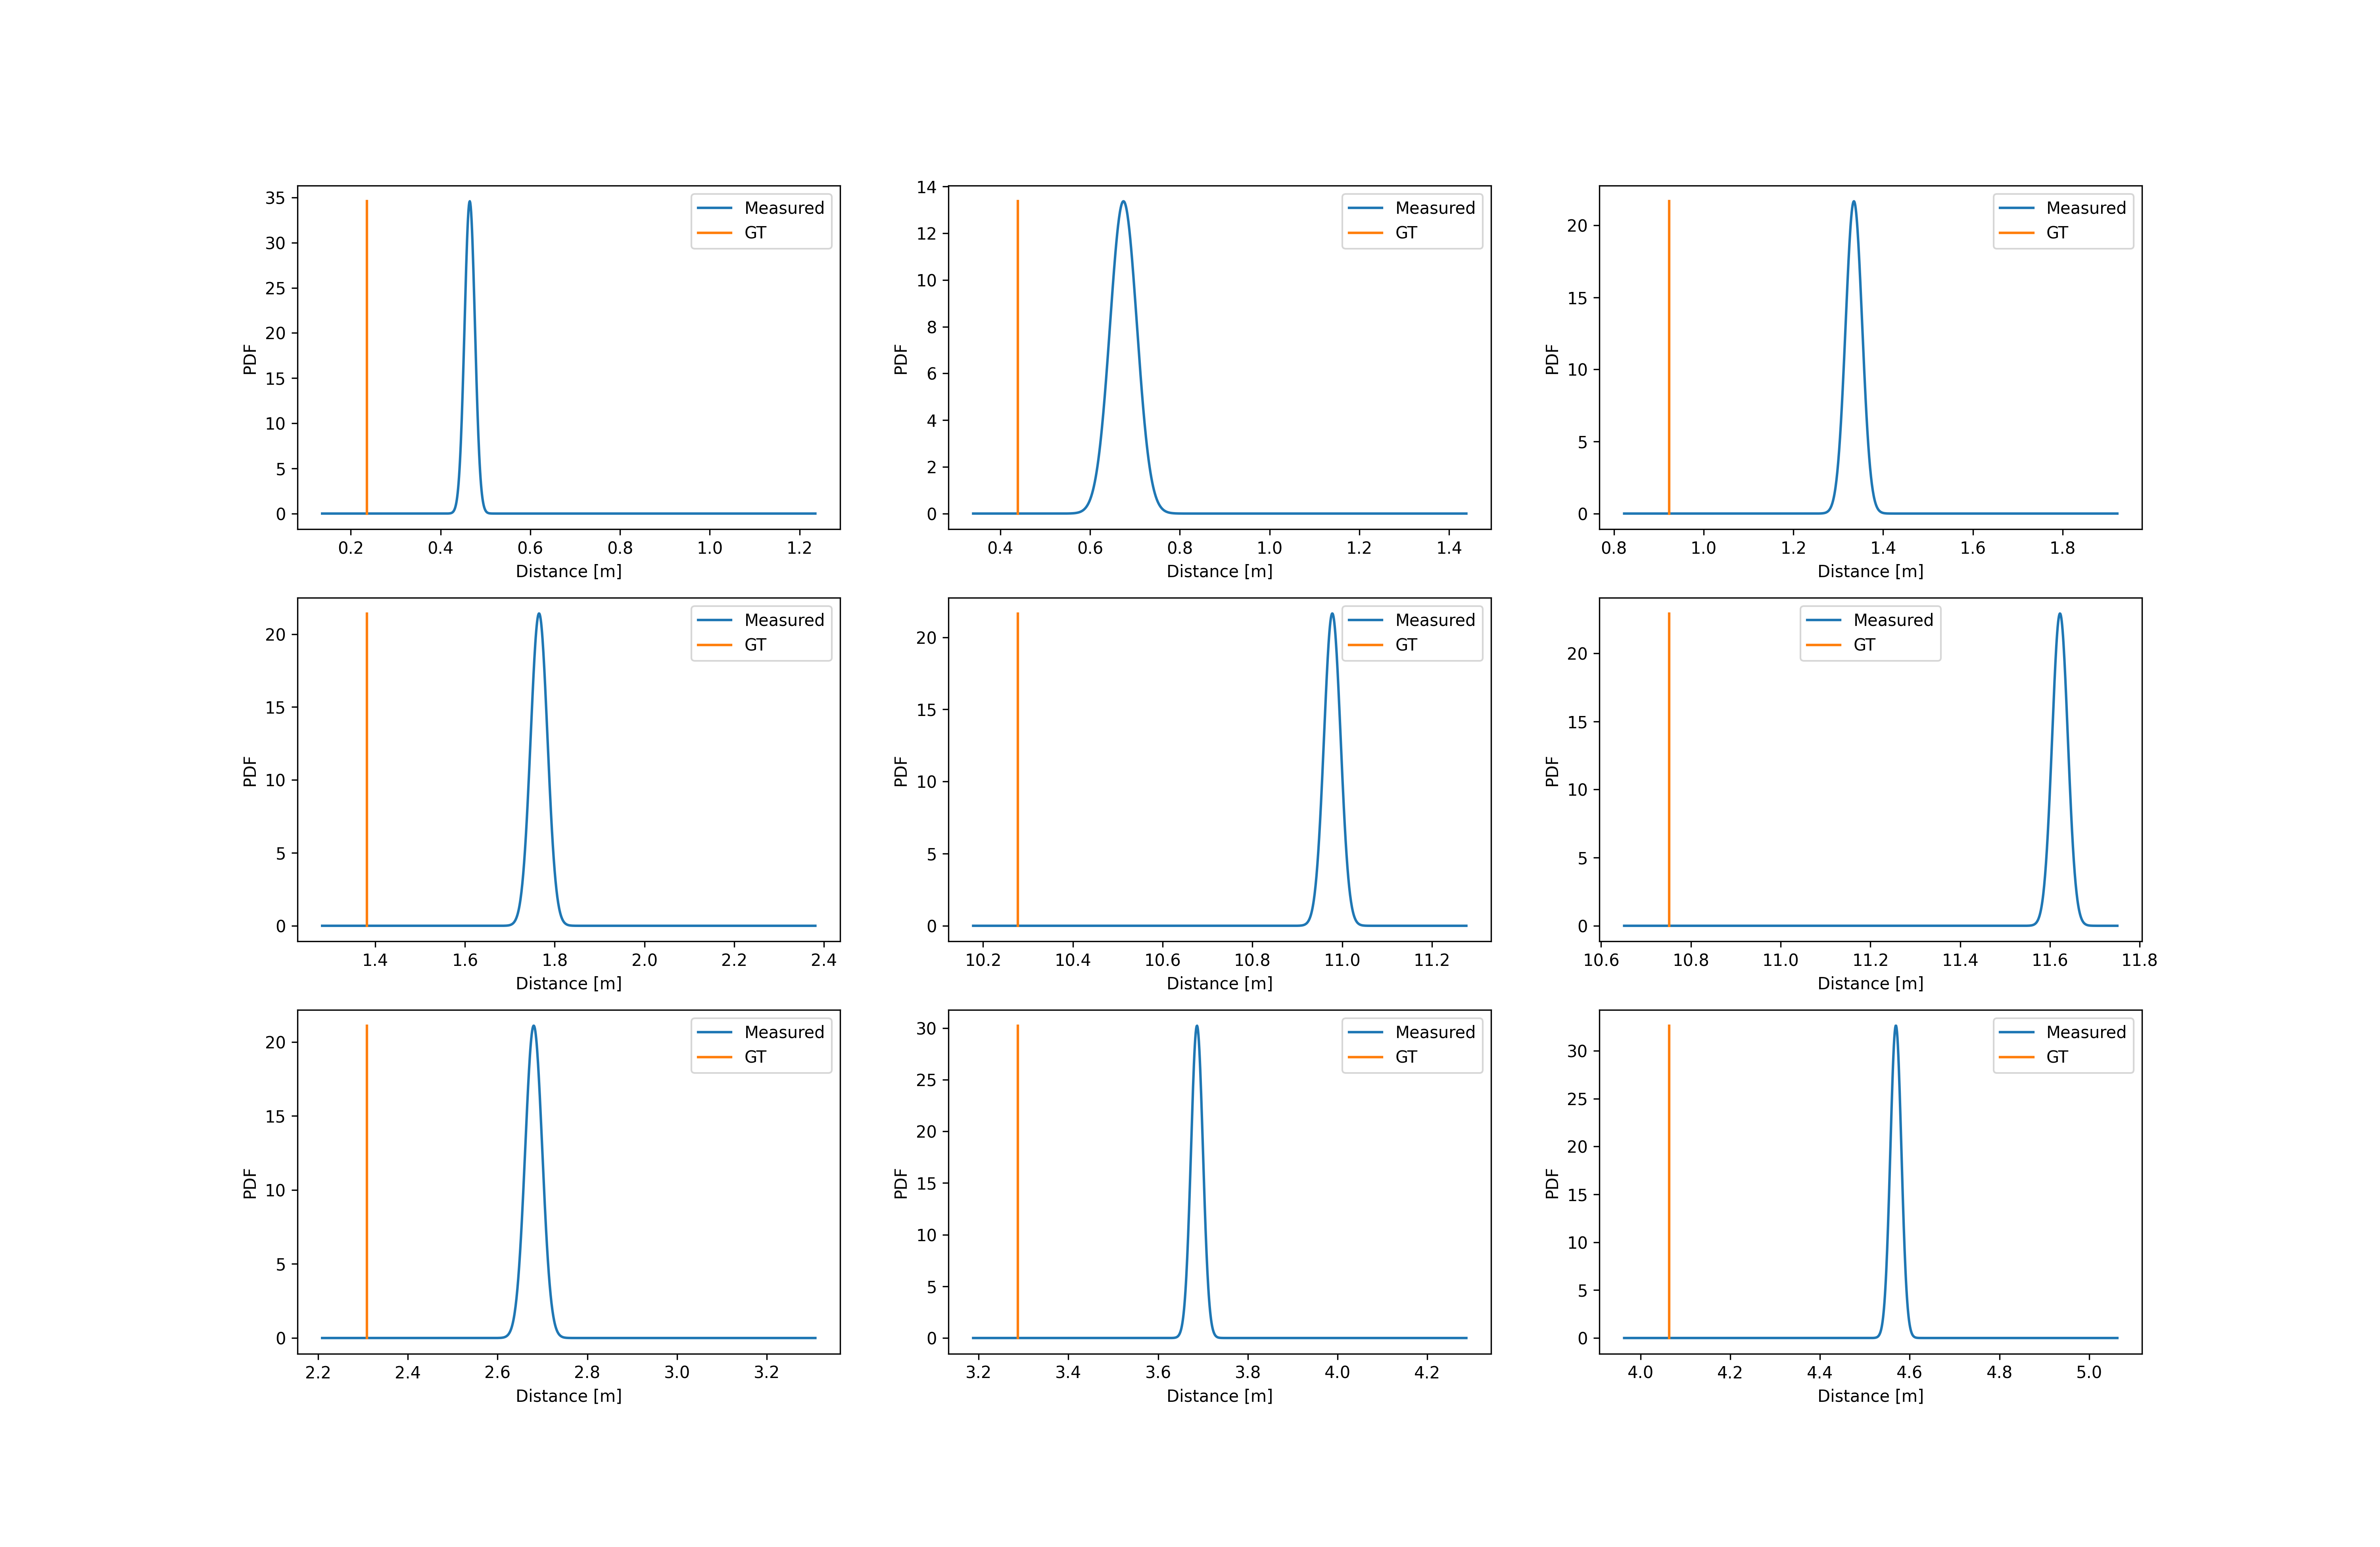
\includegraphics[width=\linewidth]{figures/distancePDF.png}
    \caption{Distance measurements PDFs.}
    \label{fig:distancePDF}
\end{figure}

Looking at the plots one noticeable thing is that mean value of measured values are shifted to the right - meaning sensor gives out bigger distance than it actually is, this could be called bias. The relationship of bias and distance is illustrated in Figure \ref{fig:distance_bias}. Additionally, it can be modeled, at least in this rang,  by a line fit, which is shown in the graph too. It approximates the bias reasonably well and will improve localization accuracy in this distance range. In a way, it's calibrating the sensor so that measurements have the same mean value as ground truths.
\begin{figure}[H]
    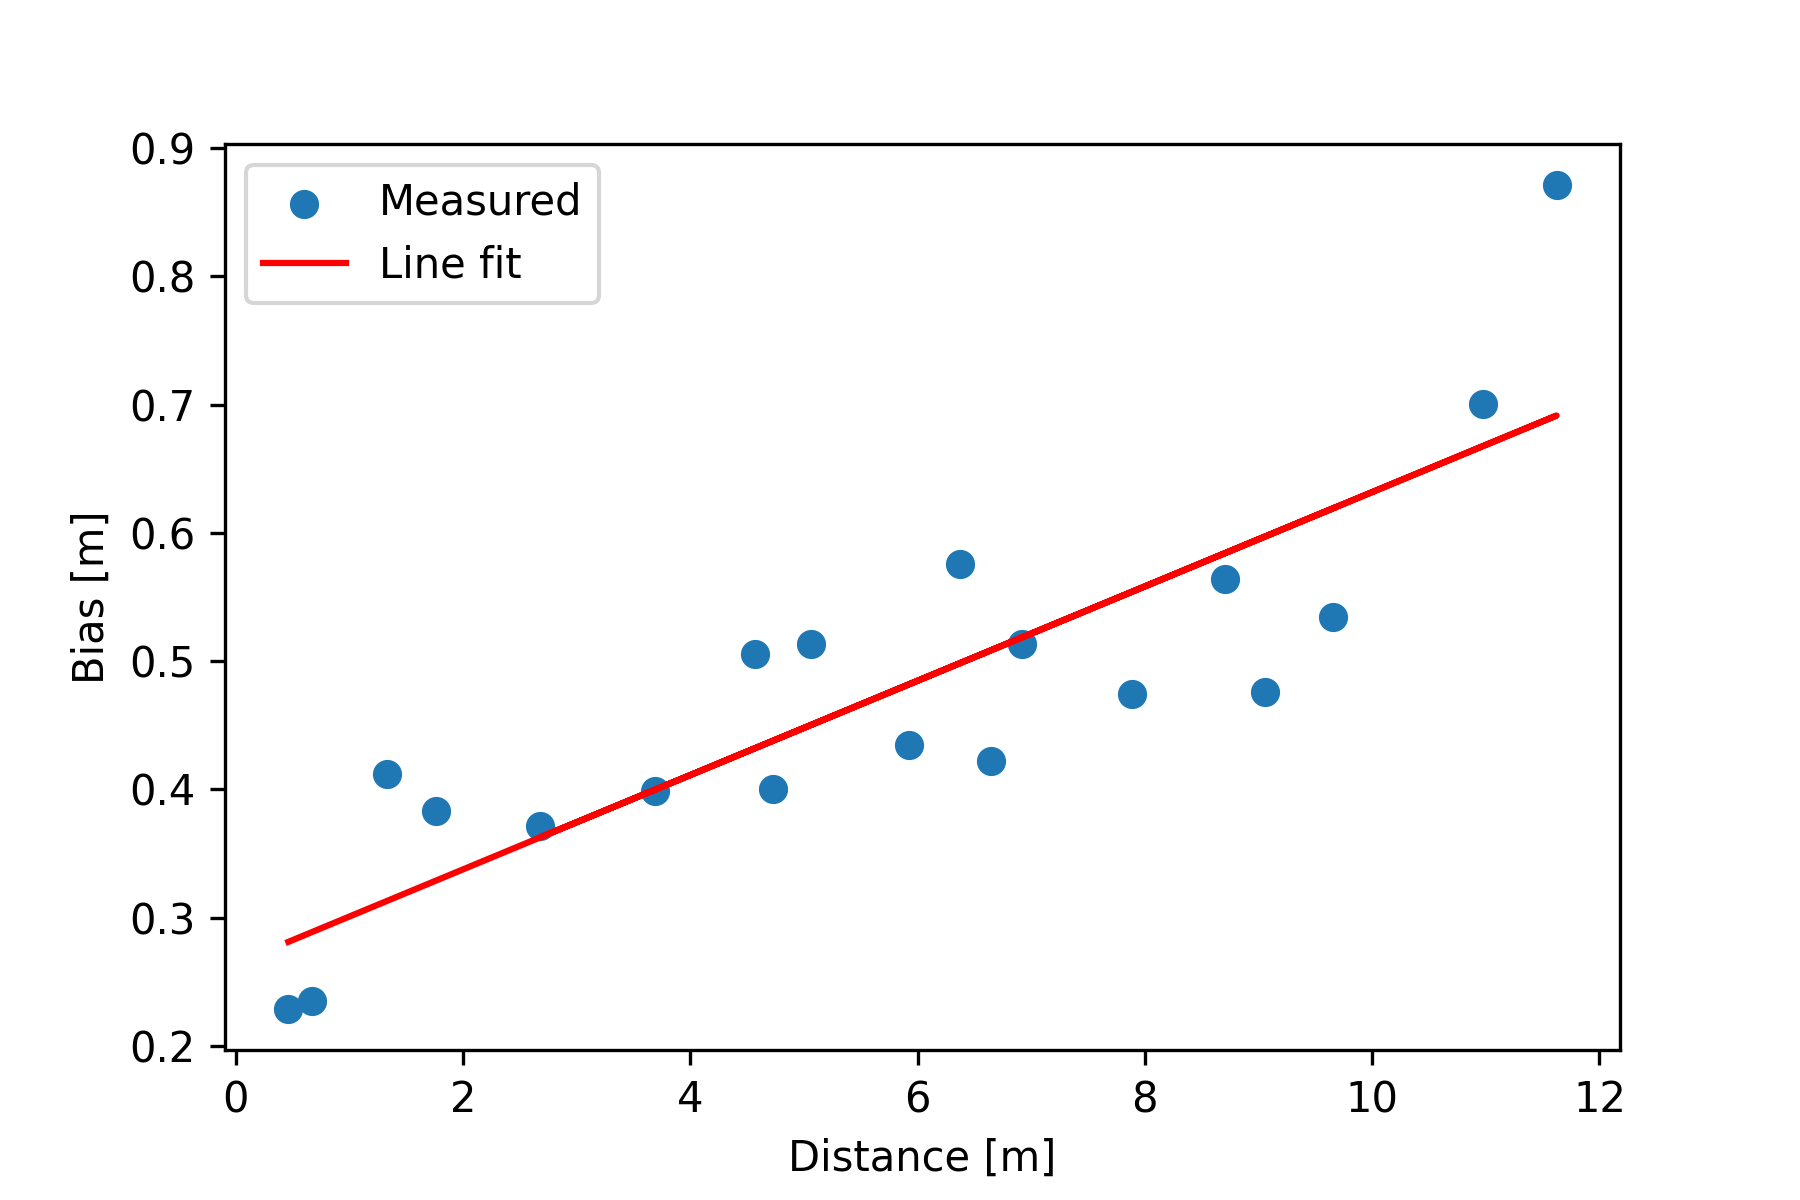
\includegraphics[width=\linewidth]{figures/distance_bias.png}
    \caption{Measurement bias over distance.}
    \label{fig:distance_bias}
\end{figure}

Next, let's look at the variance and distance relation. The question to ask here if they are dependant on each other or we can use single constant values for all range measurements. Figure \ref{fig:distance_var} shows them on single plot, plus a line fit on the data (which is, of course, bad representation of data because of one outlier). It's clearly seen that variance is very low and of almost same magnitude through out the data points. Thus, we can conclude that under tested conditions constant variance value can be used in EKF. For instance, an average value of all these variance points.
\begin{figure}[H]
    \centering
    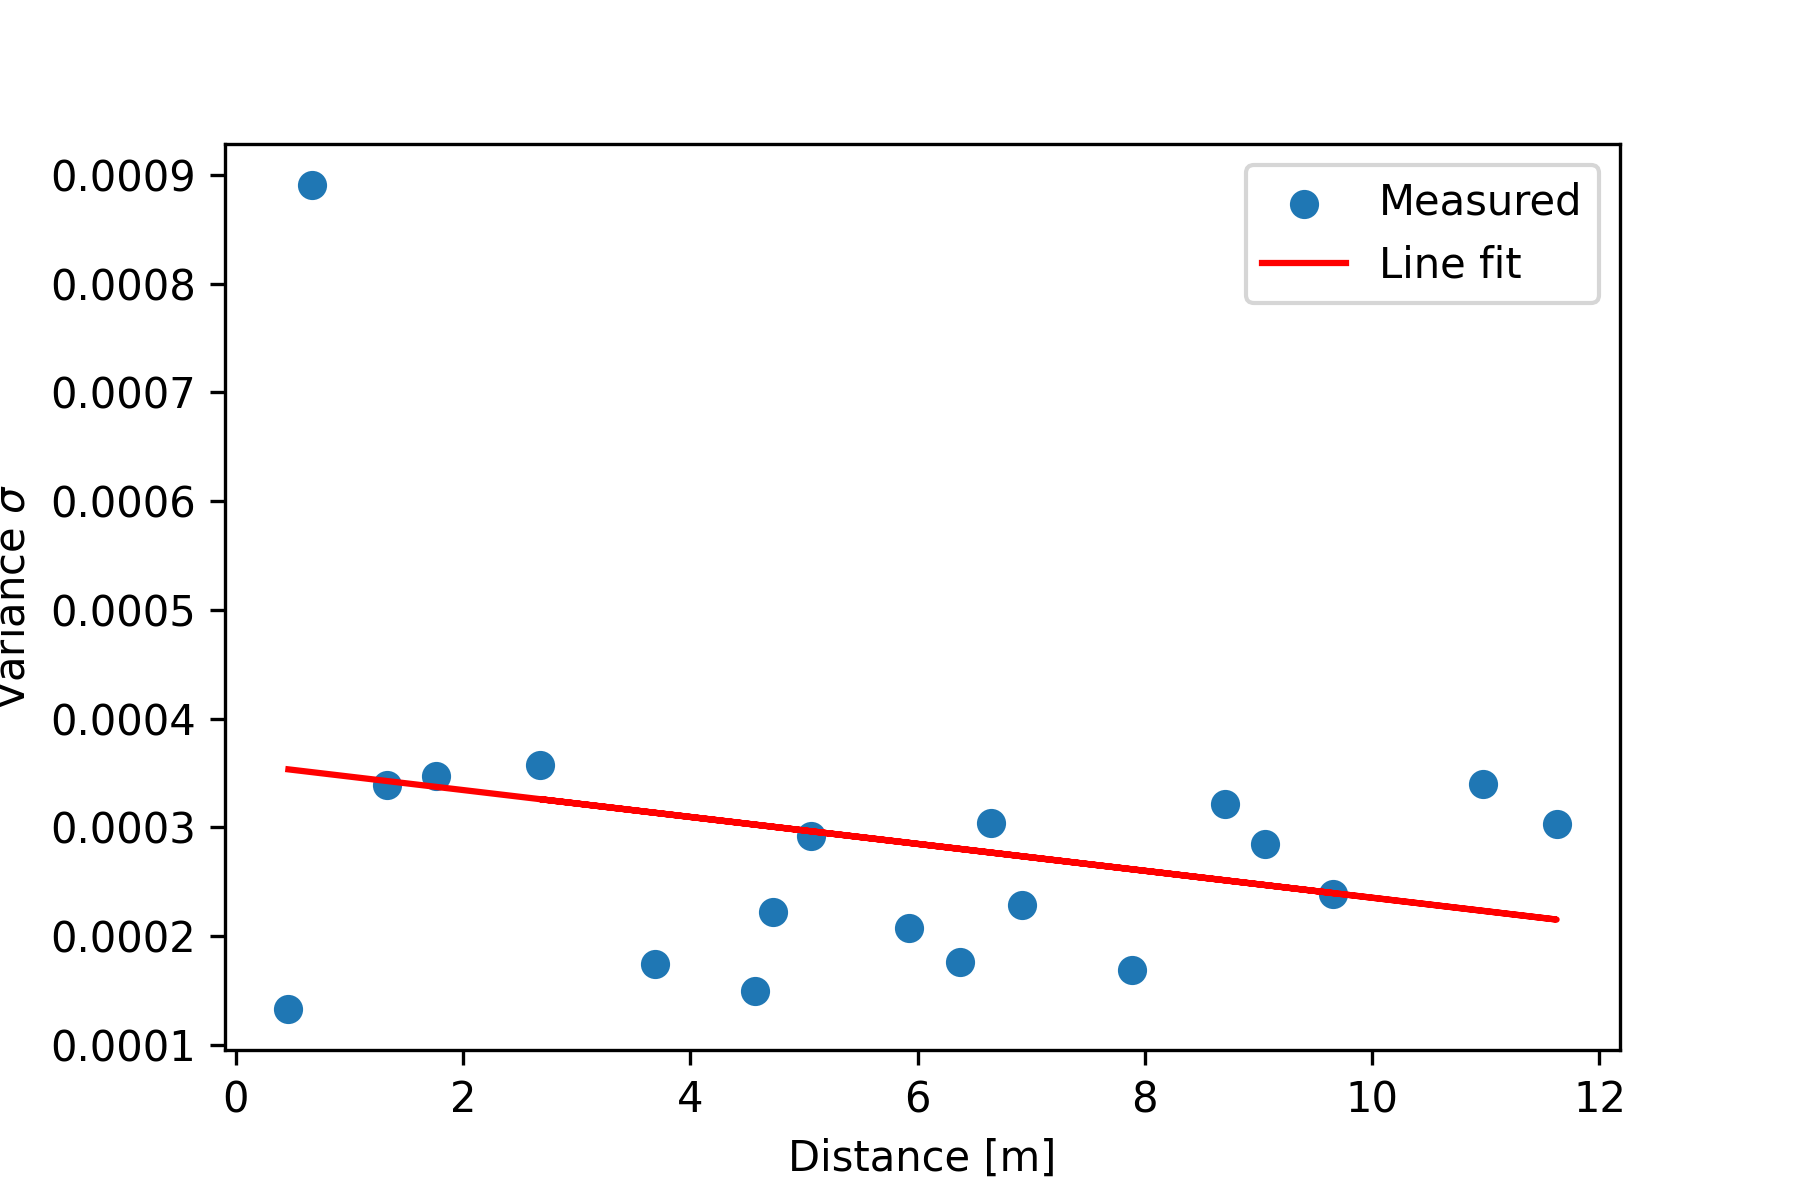
\includegraphics[width=\linewidth]{figures/dist_variance.png}
    \caption{Distance over measurement variance.}
    \label{fig:distance_var}
\end{figure}

Finally, a real experiment was conducted at DTU ASTA with Opticon system being ground truth and the setup closely following the one done in simulation i.e. having four beacons (or anchors) around an area. The tag/agent device was carried by hand to collect distance measurement from each of beacons simultaneously. Code used for data processing can be found in the root directory of repository in \emph{experiment.py} script.

It was difficult to place the beacons in different heights because of the terrain/environment thus it's expected that $z$ component of position estimate will have high variance due to lack of information. Still for validation of prototype even looking at two planar components is enough to evaluate the plausibility positioning approach using UWB antennas. At later stages this could be accounted online depending on beacon positions and possibly having more beacons to collect more information about agents position.

Also worth noting that measurement frequency is 10Hz for each beacon and connection to beacons is not stable through out the experiments, therefore measurements can be delayed or not arrive at a short enough time interval to make an update combining multiple measurements. This hints at a bigger issue - how to use data incoming at different time instances. In this case it's simply handled by a condition statements, saying that if measurement are less than some arbitrary $\Delta t$ apart in time they are considered to have occurred at the same instance in time.

Later, EKF is applied to the data colleted to reconstruct the path taken by the agent, I was trying to walk in an infinity symbol pattern. The results are depicted in Figure \ref{fig:exp_2d_path} as a planar 2D visualization with \emph{Path} being the estimated position, \emph{GT} - ground truth (Opticon), \emph{BeaconX} - beacon positions and \emph{$x0$} - the starting point of the trajectory. Figure \ref{fig:exp_3D_path} show the same trajectory in 3 dimensions.
\begin{figure}[H]
    \centering
    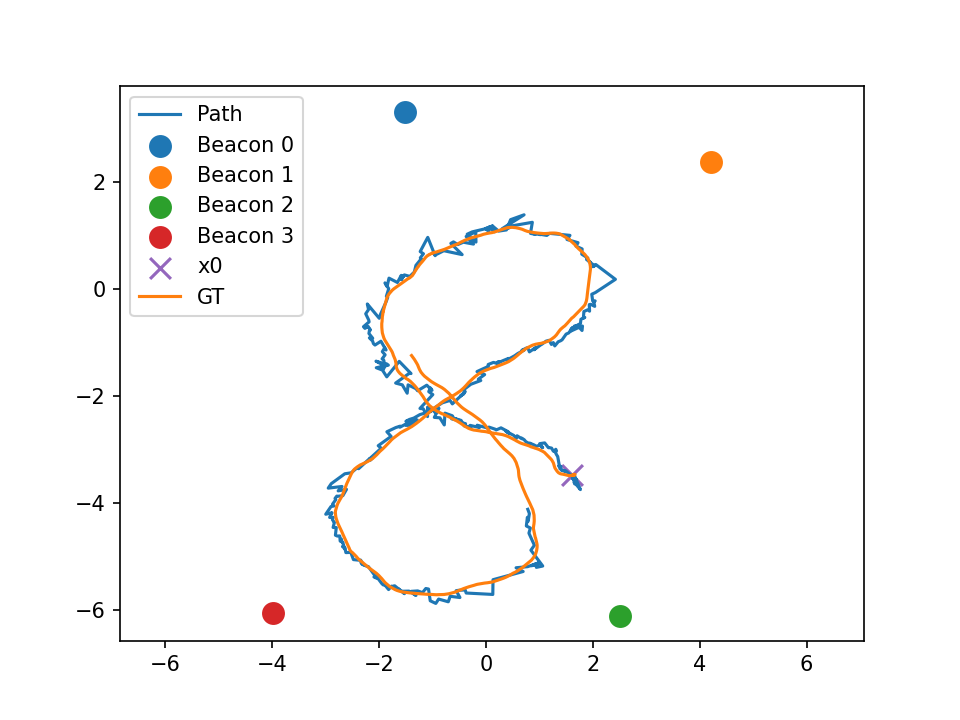
\includegraphics[width=\linewidth]{figures/2d_path.png}
    \caption{2D plot of experiment trajectory.}
    \label{fig:exp_2d_path}
\end{figure}

You can notice that trajectories are of different lengths, it's just a residual of processing because two are incoming at different rates on ROS topics and should not be mistaken as filter estimates lagging behind.

The estimated trajectory has very sharp jumps. This comes from the fact that constant velocity model used to update estimate in between measurement is very bad representation of movement in the real trajectory, especially on turns (where path is not a straight line) and whenever valid measurement arrives the estimate abruptly jumps to correct the position based on range data from beacons. When used on a real system (for instance UAV) with better system model and known input the path would be way more smooth.
\begin{figure}[H]
    \centering
    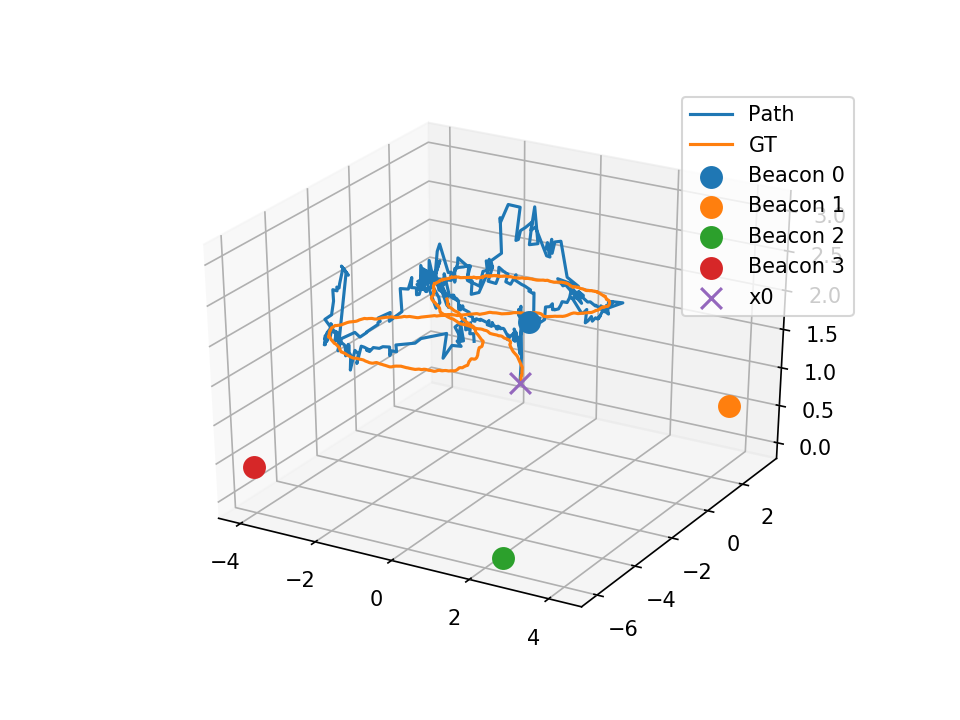
\includegraphics[width=\linewidth]{figures/3d_path.png}
    \caption{3D plot of experiment trajectory.}
    \label{fig:exp_3D_path}
\end{figure}

Futhermore it was observed that waiting for 4 measurements from all beacons to arrive at the same time is not optimal meaning if the state is updated from at least 3 measurements it already contains enough information to inform the filter about true position of agent. While doing updates from less than 3 range data points at a time was observed to negatively influence filter performance.

As expected the $z$ dimension is hardest to keep track because all of the beacons are almost in the same plane and give less information about height compared to other two directions.

Figure \ref{fig:exp_2d_path_covariances} depict the same experiment trajectory but with addition of EKF covariance plotted on top of the estimations. Important piece no notice here is that ground truth path is always in the ellipse of covariance, meaning that uncertainty accurately evaluates that estimate could be off by a certain degree and should not be trusted as is, rather should be thought as any point in the ellipse.

Following chapter will include quantitative evaluation of filter performance. The code used for obtaining metrics and plots can be found in \verb+kfeval.ipynb+ notebook.

\begin{figure}[H]
    \centering
    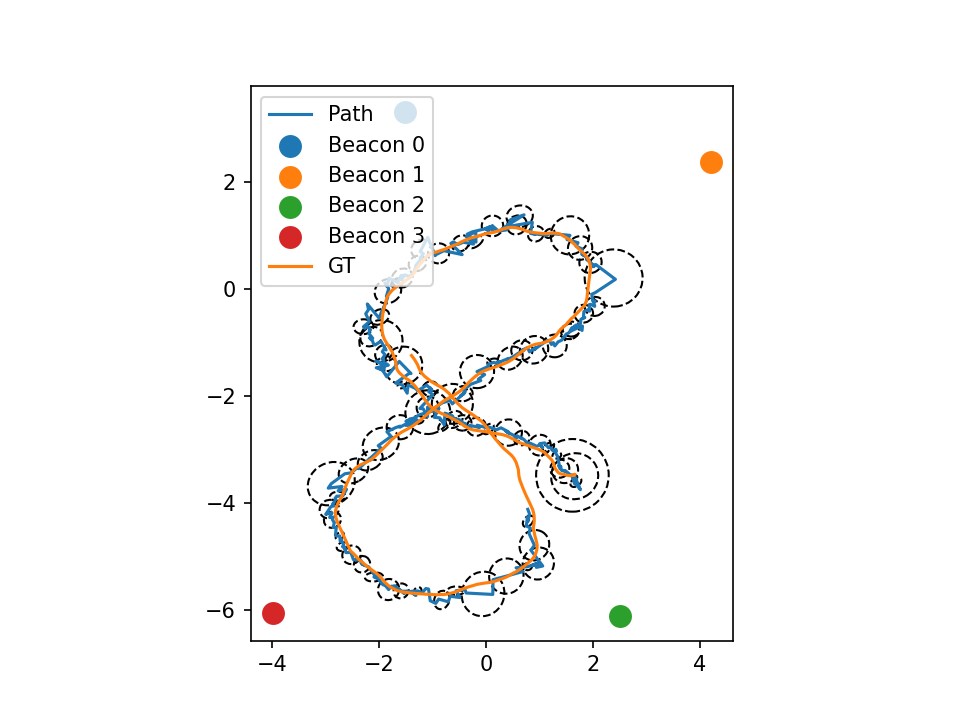
\includegraphics[width=\linewidth]{figures/2d_with_cov.png}
    \caption{2D plot of experiment trajectory with covariances.}
    \label{fig:exp_2d_path_covariances}
\end{figure}

To evaluate filter performance quantitatively several metrics can be used the most simple one could be MSE (Mean squared error), RMSE (Root MSE) or AME (Absolute mean error). But in order to compute these data points i.e. ground truth and estimated have to be aligned in time. This is not the case because Opticon system has one frequency of publishing ground truth and estimated are done in way lower frequency. Therefore each trajectory component $(x,y,z)$ are linearly interpolated in time (using \verb+scipy.interpolate+ module) to be able to select same point in time for fair comparison. For instance, Figure \ref{fig:epx_interp} shows both of them sampled from interpolated trajectories in two dimensions. Table \ref{table:error_matrics} summarizes performance of estimated trajectory quantitatively by metrics mentioned above.
\begin{table}[H]
    \centering
    \begin{tabular}{||c c c c||}
        \hline
        Metric & $x$ [m] & $y$ [m] & $z$ [m] \\ [0.5ex]
        \hline\hline
        RMS    & 0.187   & 0.132   & 0.276   \\
        \hline
        MSE    & 0.035   & 0.017   & 0.076   \\
        \hline
        AME    & 0.158   & 0.105   & 0.212   \\
        \hline
    \end{tabular}
    \caption{Error metrics.}
    \label{table:error_matrics}
\end{table}
\begin{figure}[H]
    \centering
    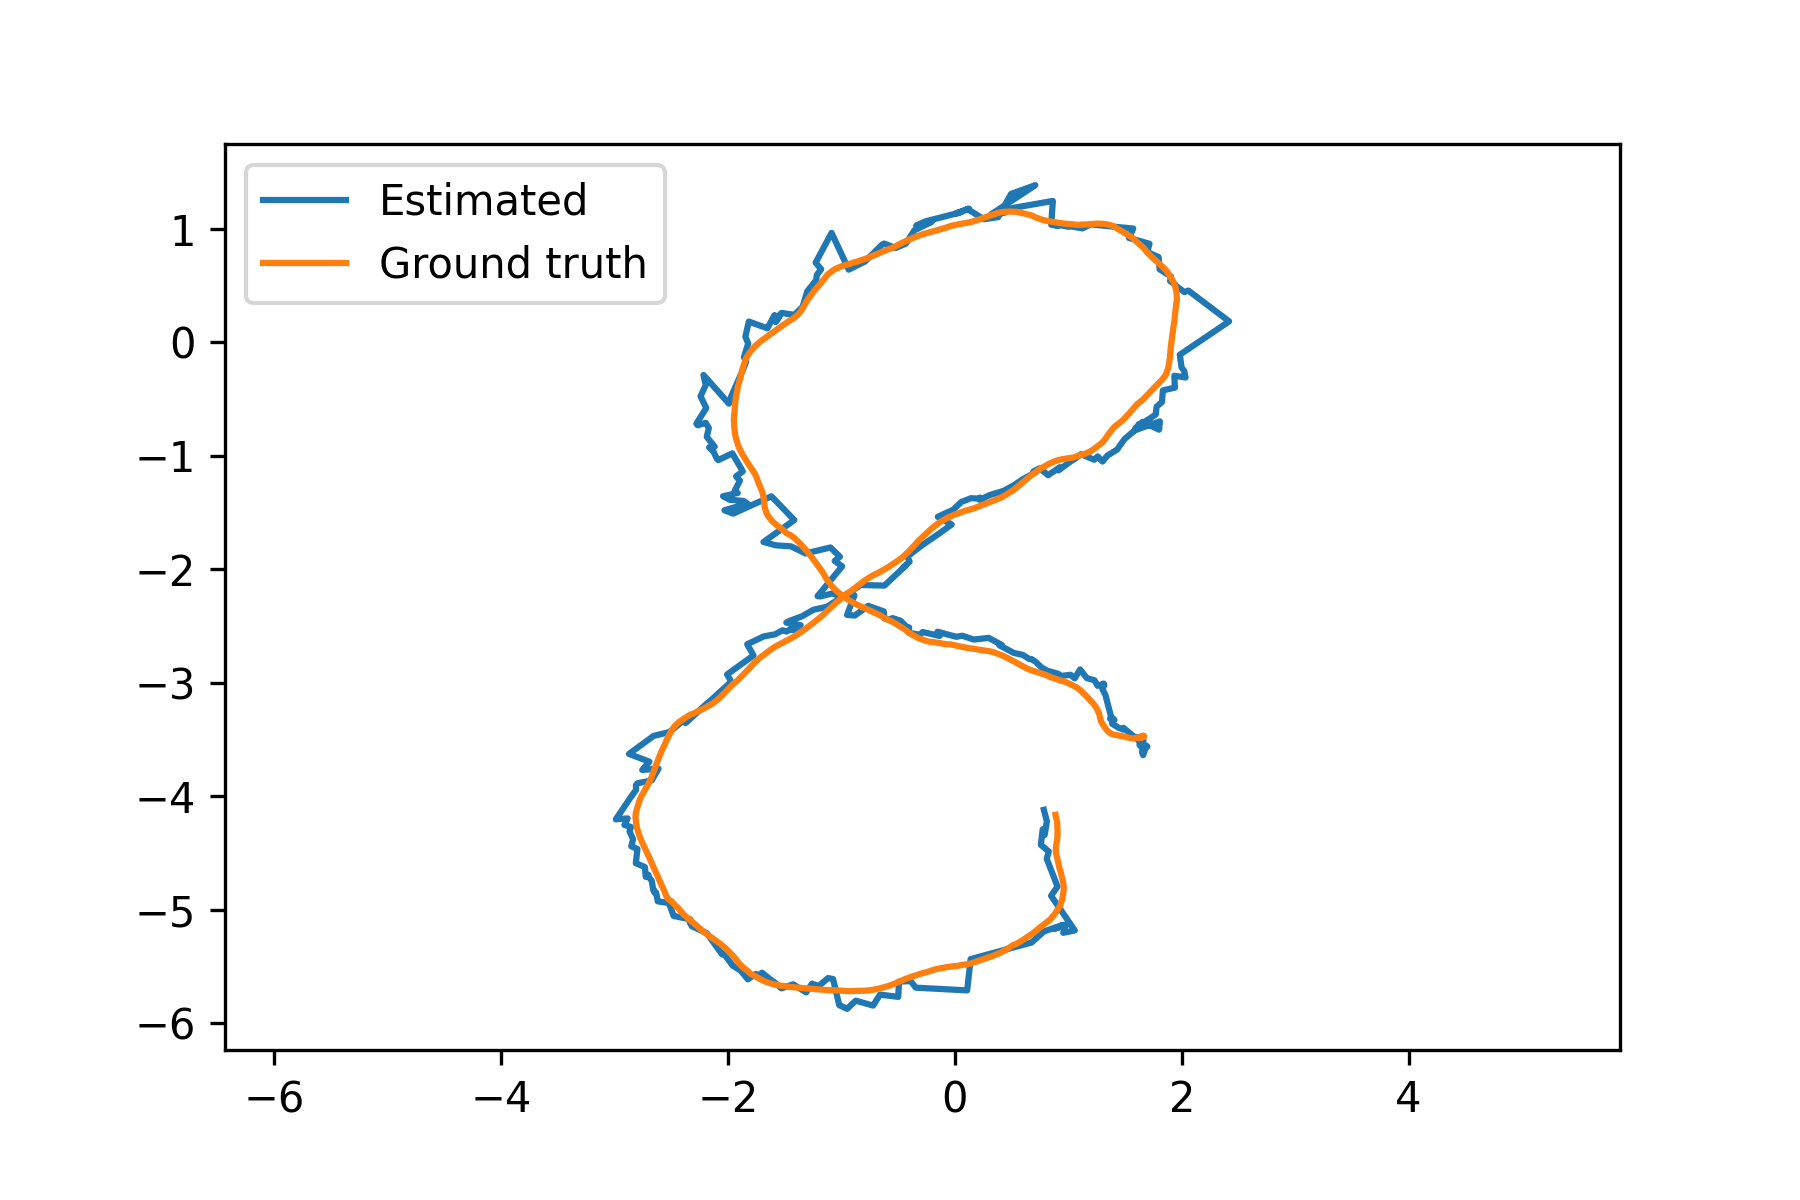
\includegraphics[width=\linewidth]{figures/interpolated.png}
    \caption{2D plot of interpolated trajectories.}
    \label{fig:epx_interp}
\end{figure}

UWB chip DW1000 datasheet \cite{dw1000chip} states that it can measure distances up to 10cm accuracy which is inline with the estimation error. Absolute mean error at least in the $(x,y)$ direction is around 10cm, the $z$ component has a bit more and reasons for it were described before.

Also Kalman Filter assumes that noise in the measurements is unbiased and white \cite{Reid2010EstimationI}. We've seen before that measurements indeed had some bias involved (it was removed before fusing data into the filter). To make sure that measures taken to remove it were effective we can plot autocorrelation function on innovation $y - \hat{y}$ and see if 95\% of the values fall into $2 \sigma$ interval i.e. $\pm 2 / \sqrt{N}$, $N$ - number of innovations. Figure \ref{fig:inno_whiteness} shows the results and indeed whiteness is confirmed. Three curves are innovation auto-correlations for each of the beacons and the bound is shown in magenta color.

\begin{figure}[H]
    \centering
    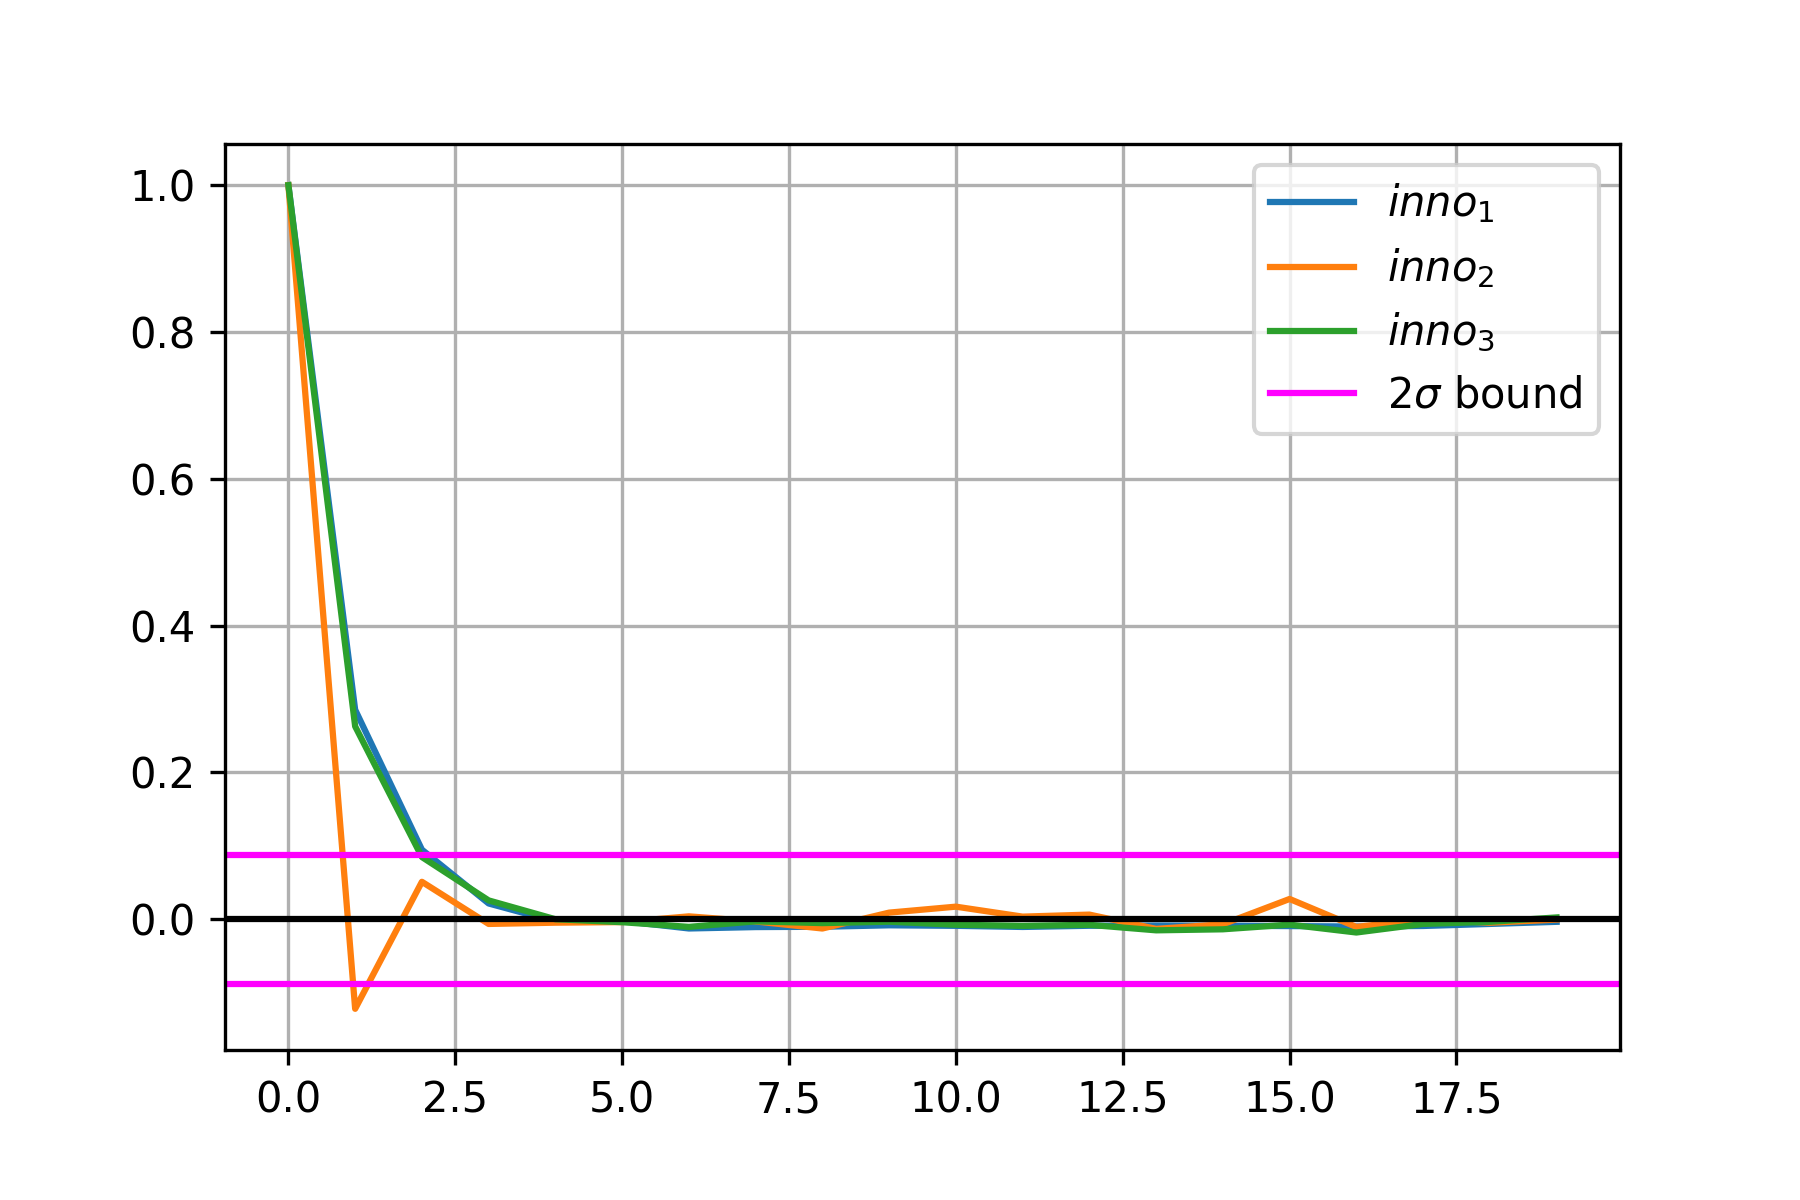
\includegraphics[width=\linewidth]{figures/inno_whiteness.png}
    \caption{2D plot of interpolated trajectories.}
    \label{fig:inno_whiteness}
\end{figure}

